\chapter{Importing Data}\label{dataload}
As discussed in section \ref{etlprocess}, the load stage of an ETL procedure can often become the most time consuming phase of the pipeline. This chapter describes the implemented procedures and examines the functionality each solution provides to complete the data load process.

\section{Put the data in databases}\label{loadsection}
The final stage in the data modelling process was to import the EMAGE and EMAPA dataset into the created data models. For each of the database systems, a different approach was required. To ensure a balanced and impartial evaluation, each of the datasets were converted into a CSV file format and manipulated by the functional tools the respective systems provide.

\subsection{MySQL}
There are various ways in which data can be loaded into a MySQL database. You can manually insert the data, row by row in the MySQL shell command prompt, using an INSERT INTO statement. However, to implement a full database using this method would be extremely time consuming and laborious. While time may not be of the essence in certain circumstances, manually writing 200,000 rows of insert statements is in no way the optimal solution to complete this task. An alternative option available is the mysqlimport command. The mysqlimport client is simply a command-line interface to the LOAD DATA INFILE statement. For readers unfamiliar with this statement, code snippet \ref{code:ldi} represents an example LOAD DATA INFILE implementation.
\newpage
\begin{lstlisting}[language=SQL, caption=Example LOAD DATA INFILE statement., label=code:ldi]
mysql > LOAD DATA INFILE '/home/callum/emageData/assay.csv'
	 	 -> INTO TABLE assays
		 -> FIELDS TERMINATED BY ','
		 -> LINES TERMINATED BY '\n'
		 -> (emageID, probeID, type);
\end{lstlisting}

The mysqlimport command can take a number of parameters some of which include, delete (empty the table before import), lock (lock all tables for writing before processing any text files) and force (continue even if an SQL error occurs). While these are useful functions, they are not required in this instance. The mysqlimport statement used to load the EMAGE dataset into MySQL can be found below in code snippet \ref{code:mysqlload}.
\begin{lstlisting}[language=SQL, caption=Command used to load data into the MySQL database., label=code:mysqlload]
---
---Import data into all tables in one command
---
mysqlimport -u root -p --ignore-lines=1 --fields-optionally-enclosed-by='"' --fields-terminated-by=',' emage assays.csv publications.csv sources.csv specimens.csv stages.csv textannotations.csv genes.csv anatomystructures.csv
\end{lstlisting}
\parindent 0pt
The command works by firstly connecting to the MySQL database as the root user and accepting a password. All of the data files I imported included headings, the ``ignore-lines=1'' parameter simply imports the data starting on line 2 thus skipping the headings row. The ''fields-terminated-by=',''' parameter allows one to stipulate the delimiter of the file, whether it be a comma, semicolon or tab for example. To signify the delimiter which encloses the values we use the parameter ''--fields-optionally-enclosed-by='"'''. The name of the database is then required to be stated in the command, hence the inclusion of ``emage''. Finally the name of the files being imported are required. When using the mysqlimport statement, multiple files can be loaded into multiple tables in one command. The name of the table is matched with the name of the file and the data is imported for each. It is therefore crucial that the ordering of the data in the file matches that of the table. If the two do not match, it is likely that \textbf{1.} The load will fail due to an incompatible data type with the values found in the file \textbf{2.} The wrong data will be mapped into the wrong columns. As each row in a CSV file is a record, there is a clear commonality between the file format and a MySQL database. Thus resulting in a relatively straightforward dataset load.
\parindent 15pt

\subsection{MongoDB}\label{mongoload}
As discussed in section \ref{mongocreate}, MongoDB documents can be created by using the \textit{db.collection.insert(\{\})} command. One simply writes a piece of valid JSON within the curly braces of this command and the document is created. This is a sleek and straightforward method however not the most efficient process available for inserting datasets of large volume.

MongoDB provides an alternative to this procedure in the form of a mongoimport tool. The mongoimport tool imports content from a JSON, CSV, or TSV file into the database. When importing a dataset which maps from your flat file into the format of your data model exactly, this method is extremely resourceful. However, should your dataset be in any other format or require structure manipulation, the mongoimport tool would not be of any use as it is a literal import. The data model I created for MongoDB includes embedded data and value arrays. As the EMAGE dataset is not in a JSON file format, using the mongoimport tool was not a feasible approach.

To load the dataset into the data model, I used the Python MongoDB API, namely PyMongo. PyMongo is a Python distribution containing tools for working with MongoDB, and is the recommended way to work with MongoDB from Python \cite{md}. The PyMongo script I created can be simply broken down into three stages; connect, insert and update. Code snippet \ref{code:pymongo} represents the full PyMongo script I wrote to load the data into the database.\\[2em]

\begin{enumerate}
\item Connect
\begin{itemize}
\item The first step is to connect to the running MongoDB instance. This is an easy step a consists of calling ``MongoClient()'' which by default connects to the host and port which is running locally.
\item We can then use the running instance to select the relevant database we want to load data into.
\end{itemize}
\item Insert
\begin{itemize}
\item To map the data into the database we create a \textit{for} loop which iterates through the CSV file.
\item The loop uses the heading of each column as the field and the row as the value. \\[2em]
\end{itemize}
\item Update
\begin{itemize}
\item To embed the Publications and Text Annotations data within the MongoDB documents I used the ``update\_ many'' command. This looks for a given value, which in this case was the EMAGE ID and updates the document with the stipulated values.
\item The ``upsert'' parameter is set to false in this instance. Upsert is the equivalent of saying ``If the value I am inserting is not currently in the database, what do I do with it?''. As I have set this to false the data will only be added if there is a match on the EMAGE ID.
\end{itemize}
\end{enumerate}
\newpage
\vspace*{\fill}
\begin{lstlisting}[language=Python, caption=PyMongo script implemented to load data into MongoDB., label=code:pymongo]
import csv

from pymongo import MongoClient

connection = MongoClient()
db = connection["mongomodel3"]
emage = db["emage"]

with open("Data/Assays.csv") as file1:
    reader1 = csv.DictReader(file1, delimiter=",")
    for row in reader1:
      emage.insert({
         '_id': int(row['emage_id']), 'probeID': row['probe_id'], 'type': row['assay_type'], 'source': row['name'], 'specimen' : {'type':row['type'],'strain' : row['strain']}, 'stage' : {'theilerstage' : int(row['theilerstage']),'dpc' : row['dpc']}})
         
with open("Data/Publications.csv") as file2:
   reader2 = csv.DictReader(file2, delimiter=",")
   for row in reader2:
      emage.update_many({'_id': int(row['emage_id'])},
         {'$push' : {'publication' : {'publicationID' : int(row['accession']), 'title' : row['title'], 'author' : row['author']}}}, upsert=False)
         
with open("Data/TextAnnotations.csv") as file3:
   reader3 = csv.DictReader(file3, delimiter=",")
   for row in reader3:
      emage.update_many({'_id': int(row['emage_id'])},
         {'$push' : { 'textannotation' : {'strength' : row['strength'], 'anatomystructure' : {'structureID' : int(row['EMAPA']),'term' : row['term']}, 'gene' : {'geneID' : row['accession'],'name' : row['name']}}}}, upsert=False)
\end{lstlisting}
\vspace*{\fill}
\newpage
\subsection{Neo4j}\label{neoload}
As discussed in section \ref{neomodel}, inserting a handful of nodes directly into a Neo4j database is relatively straightforward. All that is required are a few commands and you can have a fully functioning data model. For a detailed description on how to do this see section \ref{neomodel}. However, this is on a small scale only. The process for implementing a full data model with a large dataset requires more resource.

The query language which Neo4j is based on, Cypher Query Language, allows for multiple ways of implementing a data model. The main way to do this is to use Cypher's LOAD CSV command to transform the contents of a CSV file into a graph structure. Code snippet \ref{code:cypher} represents the Cypher file created to load the Assay nodes into the Neo4j database. %The full Cypher file can be found in appendix \ref{app:cypher}.

The main structure of the query and the commands used are similar for the two approaches. However, to load data in via a CSV one requires two additional lines, these are represented in lines 5 and 6 of code snippet \ref{code:cypher}. Line 5, ``USING PERIODIC COMMIT'' is used when loading large amounts of data in a single cypher query. This is because loading large volumes of data within a single query runs the risk of failing due to running out of memory. Thus including this function prevents the query failing for this reason. However, it will also break transactional isolation and should only be used where needed \ref{neo}. Line 6 of code snippet \ref{code:cypher} simply loads the file found at the stipulated location and assigns it to a variable name, ``row'' in this case.

One additional noteworthy aspect of code snippet \ref{code:cypher} is the use of the ``MERGE'' keyword. MERGE either matches existing nodes and binds them, or it creates new data and binds that. MERGE is like a combination of MATCH and CREATE that additionally allows you to specify what happens if the data was matched or created \cite{nd}. Semantically it is the same command as the MongoDB ``upsert'', as discussed in section \ref{mongoload}. Using this keyword aids the normalisation process.
\newpage
\vspace*{\fill}
\begin{lstlisting}[language=SQL, caption=Cypher file created to load assay data into the Neo4j data model., label=code:cypher]
CREATE CONSTRAINT ON (e:Assay) ASSERT e.id IS UNIQUE;
CREATE INDEX ON :Assay(emageID);

// Create Assays
USING PERIODIC COMMIT
LOAD CSV WITH HEADERS FROM "file:/home/callum/Documents/Uni/F20PA/Project/Neo4j/Data/Assays.csv" AS row

// Query the already created nodes and match them based on the following clauses.
MATCH (source:Source {sourceID : TOINT(row.source_id)})
MATCH (specimen:Specimen {specimenID : TOINT(row.specimen_id)})
MATCH (stage:Stage {stageID : TOINT(row.stage_id)})

// Create Assay nodes.
MERGE (assay:Assay {emageID: TOINT(row.emage_id)})
SET assay.probeID = row.probe_id, assay.type = row.type

// Create Assay relationships.
CREATE (assay)-[:COMES_FROM]->(source)
CREATE (assay)-[:CLASSIFIED_AS]->(specimen)
CREATE (assay)-[:GROUPED_BY]->(stage);
\end{lstlisting}
\vspace*{\fill}
\newpage

\subsection{Apache Cassandra}
There are a number of ways in which one can load a preformed dataset into a Cassandra cluster. In the early days of Cassandra, a low level interface, BinaryMemtable was used to ingest data. However, this tool was deemed rather difficult to use and is now defunct functionality \cite{cass}.

Other tools which are available are json2sstable and sstableloader. While these alternatives are thought to be extremely efficient and powerful for importing millions of rows of data, they require careful network and configuration considerations \cite{cass}. Thus, making the process unnecessarily complicated for the programmer. For situations such as this, where either the volume of data does not merit the use of sstableloader, nor learning the use of json2sstable is deemed a valuable use of resource, another alternative is available; COPY FROM.

The COPY FROM command is used on the Cassandra cqlsh interface. Cqlsh is a python-based command prompt for executing Cassandra Query Language (CQL) queries \cite{ds}. The usefulness of this command is that it accepts CSV data. COPY FROM accepts a number of parameters which allows the programmer to specify exactly what format the CSV file is in. While a CSV file type is recognised as a common format, there is no one way of structuring the file. By this I mean, a file can have headers, varying escape characters, different delimiters and multiple character encodings. All of which can be specified using the COPY FROM command parameters.

\begin{lstlisting}[language=SQL, caption=Loading data into Apache Cassandra using the cqlsh interface., label=code:cass]
---
--- Copy the EMAGE submissions data into the assays table.
---
COPY assays (emageID,assayType,dpc,probeid,source,specimenstrain,specimentype,theilerstage)
FROM '~/Desktop/emage_submissions.csv'
WITH DELIMITER = ','
AND HEADER = TRUE;
\end{lstlisting}

Code snippet \ref{code:cass} represents the loading of the Assay data into the assays table using the COPY FROM command. The command requires you to state the name of the table you are loading data into; ``assays'' in this example. Then specify the column names you will be importing data into in brackets.  The important thing to remember when using the COPY FROM command on a CSV file is that the ordering of the file headings must match the ordering of the columns in the table. Cassandra does not offer any way of mapping file headings to table column names. Therefore if there is a misalignment of data columns the values will be loaded incorrectly, and more often than not the load will fail due to incompatible data types. The FROM keyword denotes the location of the CSV file you will be loading. The WITH clause allows you to impose any rules on the COPY FROM command. In this instance, I have stipulated the delimiter of the file as a comma, and that there are headings in the top row of the file. After you run this command, the data will have been imported into the Cassandra tables.
\newpage
\section{Discussion}\label{loaddiscussion}
Each system provides the relevant functionality to insert data into the databases on both a large and small scale. Using the query language of each system, inserting data manually is done by using a variation of the SQL INSERT INTO statement. This functionality is seen as one of the minimum requirements for a database management system. While each of the solutions have their own twist on how the physical load is done, they are all relatively similar.

One of the key aspects of a NoSQL system is the flexibility it offers. The main reason for this is because NoSQL systems are schema-less. The benefit of this attribute is nevermore apparent than when loading data into a data model. Creating the optimum data model for a system can often be a trial and error exercise. Thus being able to modify and manipulate your system architecture easily is a big advantage. Where many NoSQL systems differ from relational databases systems such as MySQL is that the schema is created at the time of load. Such is the case for MongoDB and Neo4j. While I had created diagrams to visualise the structure of these systems, the physical schema had not been implemented. Consequently, some changes to the final schema were made after the data had been loaded into the databases. Because the systems schema is completely dynamic and flexible I was able to add, remove and update fields with ease. For example, if I were to add an additional piece of information for say a specific document (in MongoDB) or node (in Neo4j) I could just use the relevant insert statement and the data is loaded into the database. Comparatively if I were to do this in a MySQL structure, I would have to add an entire column and update appropriately. For just additional field I would have an entire row of null values. This is computationally more expensive and is also more time consuming. If we look at Cassandra, we again have to add an entire column, however we do not have null values. Therefore we can add additional data freely, at very little resource cost. This is certainly a big advantage of using a NoSQL system.

One of the main objectives of this project was to analyse the performance of the database solutions. The term performance covers a wide range of components and can be measured in many ways. For this stage of the project the \textit{load} performance of the systems was something which I was interested in analysing. It is rarely the case where an entire database of information will be inserted at any one time. However, if one is looking to migrate from one database management system to another or a database is being restored from a backup for example, the time it takes to physically load the data is something which should be taken into consideration. Therefore I created an experiment to evaluate the total time it takes to load the data into the respective solutions.

The purpose of the experiment was simple, to identify the system which loads the EMAGE dataset into the data model in the quickest time. More precisely, I was looking to identify the affect imposing indexes and unique/distinct constraints had on the time taken to load data. For each of the solutions, the test was considered complete once each of the insert statements was finished and the databases were fully populated. Once a query was run on each of the systems, the execution time was printed on the command-line. This time was used to measure the outcome of the test. To enhance the fairness of the experiment, each query was run 5 times, with the average time across the tests recorded. After each run, the contents of each of the databases was removed, resulting in empty systems.

\begin{table}[H]
\centering
\begin{tabular}{|c|c|}
\hline
\textbf{Hardware/Software} & \textbf{Specification} \\ \hline
Computer Model & Dell Inspiron 1545 \\ \hline
Operating System & Ubuntu 15.10 \\ \hline
Processor & 2.3 GHz Pentium(R) Dual-Core \\ \hline
Physical Memory (RAM) & 6Gb \\ \hline
Storage & 512 GB SSD \\ \hline
Graphics & Intel Integrated GMA 4500 MHD \\ \hline
\end{tabular}
\caption{Machine configuration}
\label{tab:sysspec}
\end{table}

Table \ref{tab:sysspec} above, outlines the system specification which the data models were created in. Each of the database solutions were run locally on the same machine. The idea of this table is to aid the reader when discussing the performance of the solutions and allow one to understand the underlying hardware and software behind the systems.

\subsection{Experiment 1}\label{experiment1}
The first step in creating the experiment was to implement the data models so I could load in data. As the MongoDB and Neo4j schemas are dynamically created, this step was only possible for the MySQL and Cassandra systems. A full discussion on the schema implementation stage can be found in chapter \ref{implementation}. The time taken to create the schemas was not taken into consideration when measuring the execution time. The timings were purely based on the time taken to run the import statements.

As one of the main aims of this experiment was to identify the affect of implementing indexes pre-load had on import time, I only created the tables. Indexes and unique constraints were not applied until after the data was loaded. Primary and foreign keys were applied for the MySQL model. For the Cassandra system, partition and clustering keys were implemented where necessary. To create the test for the MongoDB and Neo4j systems, I initially loaded the data into the databases and did not apply any indexing or unique constraints.

One can use indexing in a database to find data rows with specific column values quickly; much like the indexing of a book. The intention of this is to improve the performance of commonly run queries. Intuitively, one would expect quicker load times and a slower querying performance with no indexes implemented. A number of behaviours should be taken into consideration when deliberating system performance. Factors such as the impact on write operations and the amount of space each index requires can have a profound affect on the execution of queries. Another consideration is the size of files being loaded. The volume being loaded into the MySQL and MongoDB solutions was around 12mB and the Neo4j data model was loaded with around 20mB of data. For the Cassandra system, the size of the files being loaded cumulatively came to around 35mB. This was as a result of each of the systems using a normalised model compared to the Cassandra database. If one was to compare the database solutions directly, this is a component which would need to be taken into consideration. However, this experiment was to analyse the affect of implementing indexes and unique constraint as opposed to solely focusing on which system loads the data in quickest time.

Once the tables were created, the next step was to load the data into the systems, using the various import commands. The results of the initial experiment can be found in table \ref{tab:l1}. These values represent the load times for non-indexed database systems. The load times 

\begin{table}[H]
\centering
\resizebox{\textwidth}{!}{
\begin{tabular}{|c|c|c|c|c|c|c|c|}
\hline
\textbf{Database System} & \textbf{Version} & \textbf{\begin{tabular}[c]{@{}c@{}}Load 1\\ time (s)\end{tabular}} & \textbf{\begin{tabular}[c]{@{}c@{}}Load 2\\ time (s)\end{tabular}} & \textbf{\begin{tabular}[c]{@{}c@{}}Load 3\\ time (s)\end{tabular}} & \textbf{\begin{tabular}[c]{@{}c@{}}Load 4 \\ time (s)\end{tabular}} & \textbf{\begin{tabular}[c]{@{}c@{}}Load 5\\ time (s)\end{tabular}} & \textbf{\begin{tabular}[c]{@{}c@{}}Average load\\ time (s)\end{tabular}} \\ \hline
\textbf{MySQL} & 5.7.11 & 5.20 & 5.14 & 5.16 & 5.25 & 5.33 & \textbf{5.21} \\ \hline
\textbf{MongoDB} & 3.2.4 & 127.5 & 186.9 & 152.4 & 159.7 & 133.8 &  \textbf{152.06} \\ \hline
\textbf{Neo4j} & 2.3.3 & 20594.09 & 20234.41 & 20911.35 & 20198.70 & 20121.86 & \textbf{20412.08} \\ \hline
\textbf{Apache Cassandra} & 3.0.4 & 189.47 & 165.11 & 168.69 & 182.33 & 161.85 & \textbf{173.49} \\ \hline
\end{tabular}}
\caption{Load times for non-indexed database systems}
\label{tab:l1}
\end{table}

\parindent 0pt
remained consistent throughout each of the tests. This gives rise to eliminate any concerns regarding simultaneous processes running on the computer, affecting the performance of the experiment.
\parindent 15pt
If we look at the systems individually, the MySQL load times were extremely fast at just 5 seconds. While not quite as impressive but still a reasonable time, the MongoDB model managed to load the data in around 2.5 minutes. Comparatively the Cassandra database loaded all of the data in just under 3 minutes. This time is all the more impressive when you consider the fact that the Cassandra model was loading almost 3 times the data as that of the MySQL and MongoDB systems. Figure \ref{fig:loadvsfile} illustrates the time taken to load the data against the volume of data being uploaded.
\begin{figure}[H]\begin{center}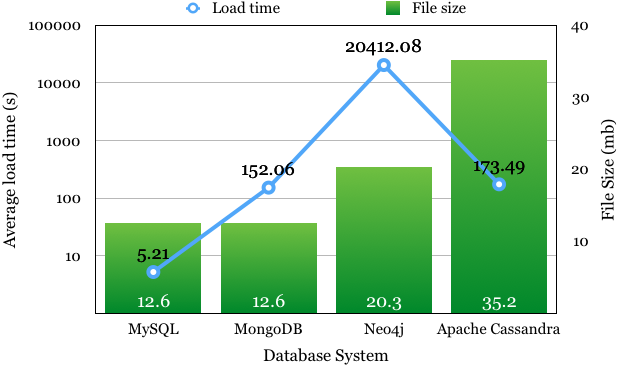
\includegraphics[width=1\linewidth]{images/loadvsfile}\caption{Chart illustrating the variance in load times of non-indexed systems vs the file size}\label{fig:loadvsfile}\end{center}\end{figure}

As you can see from the graph, the MySQL system is running the import statements at a rate of around 2mB per second. The MongoDB system is importing the data at a rate of around 800kB per second. The Cassandra system is running the import commands at a rate of around 200kB per second. As the Neo4j system is evidently uncomprehendingly slow, the time taken to import the data is disregarded for this comparison.

The most striking result of the experiment was the Neo4j system taking on average around 5.5 hours to complete. That is 117 times slower than the next longest running load time of the Cassandra system and a staggering 3917 times slower than the fastest MySQL database. For an in-depth discussion on the findings of this experiment, see section \ref{experimentdiscussion}. Before moving on to the next stage of the experiment it is worthwhile making some assumptions about the results of test 1.

\begin{itemize}
\item As the MySQL tables have been normalised and structured adequately, the system can write a high number of rows at very high speed.
\item By default the MongoDB model uses the \_id field as a sort of indexed primary key. Therefore after every insert or update operation, MongoDB must update every index associated with the collection in addition to the data itself. Thus increasing the amount of overhead for the performance of write operations.
\item Neo4j model is struggling to process the high number of reads compound with the writes when matching the relationships simultaneously.
\item The Cassandra system is processing a reasonable level of operations for a larger volume of data.
\end{itemize}

\subsection{Experiment 2}\label{experiment2}
The next stage of the experiment was to implement the indexes and unique constraints on the data models. The processes for imposing these operations are discussed in chapter \ref{implementation}, section \ref{dbcreate}. The structure of the solutions was the same as that of the first experiment. All of the conditions were repeated in the same manner as before. It was important that I recreated the setup for the second test as close as possible to that of the first test. As a result, I was able to analyse and examine the results closely allowing me to draw interesting and accurate conclusions. The overall aim of the second experiment was to identify any changes in load performance when imposing indexes on the solutions. The result of running the second experiment can be found in table \ref{tab:l2}.

\begin{table}[H]
\centering
\resizebox{\textwidth}{!}{
\begin{tabular}{|c|c|c|c|c|c|c|c|}
\hline
\textbf{Database System} & \textbf{Version} & \textbf{\begin{tabular}[c]{@{}c@{}}Load 1\\ time (s)\end{tabular}} & \textbf{\begin{tabular}[c]{@{}c@{}}Load 2\\ time (s)\end{tabular}} & \textbf{\begin{tabular}[c]{@{}c@{}}Load 3\\ time (s)\end{tabular}} & \textbf{\begin{tabular}[c]{@{}c@{}}Load 4 \\ time (s)\end{tabular}} & \textbf{\begin{tabular}[c]{@{}c@{}}Load 5\\ time (s)\end{tabular}} & \textbf{\begin{tabular}[c]{@{}c@{}}Average load\\ time (s)\end{tabular}} \\ \hline
\textbf{MySQL} & 5.7.11 & 8.10 & 9.45 & 8.32 & 8.15 & 8.37 & \textbf{8.47} \\ \hline
\textbf{MongoDB} & 3.2.4 & 370.80 & 342.11 & 347.50 & 393.82 & 366.25 & \textbf{364.09} \\ \hline
\textbf{Neo4j} & 2.3.3 & 175.03 & 121.54 & 128.0 & 145.62 & 120.41 & \textbf{138.12} \\ \hline
\textbf{Apache Cassandra} & 3.0.4 & 203.16 & 241.01 & 285.97 & 279.40 & 281.36 & \textbf{258.18} \\ \hline
\end{tabular}}
\caption{Load times for indexed database systems}
\label{tab:l2}
\end{table}
Table \ref{tab:l2} shows the variance in load time after implementing indexes on the database solutions. Again there is a consistency in each of the execution times. With the exception of Neo4j, each of the solutions saw an increase in load time. The MySQL system took around 3 seconds longer. The time taken for the MongoDB model to load the data more than doubled and the Cassandra system took around a minute longer. Figure \ref{fig:nonvsin} below illustrates the increase in load time of non-indexed vs indexed database solution. This bar chart shows the

\begin{figure}[H]\begin{center}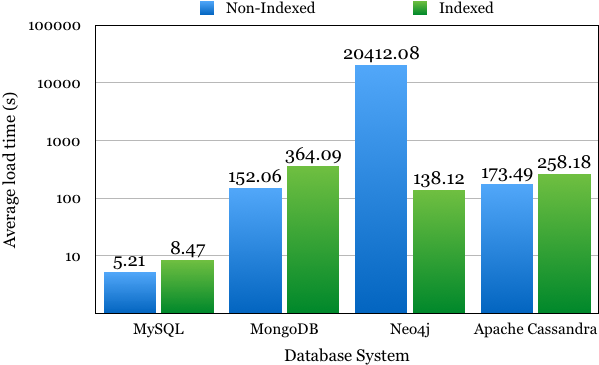
\includegraphics[width=1\linewidth]{images/nonvsin}\caption{Chart illustrating the variance in load times of non-indexed vs indexed systems}\label{fig:nonvsin}\end{center}\end{figure}
\parindent 0 pt
affect implementing indexes has on the load time of data models. These findings posed the question, why did this alteration cause such a drastic affect. One detail which must be taken into consideration when evaluating these results is the fact that the experiment was not just to purely load raw CSV data into the solutions. The data was being loaded and modelled concurrently, in a way in which I believed would result in the most performant system. Therefore, in the cases of MongoDB and Neo4j, I used update\_many and MATCH statements to create the relationships in the data. This added significant computational resource and time to the overall load process. In contrast, for the MySQL and Cassandra solutions, as I had already created the table structures, I was able to directly load the data, without having to query the rest of the database.\parindent 15 pt

\subsection{Experiment evaluation}\label{experimentdiscussion}
The official MongoDB documentation suggests that there are a number of operational considerations when implementing indexes. For example, they state that ``Each index requires at least 8kB of data space.'' and ``Adding an index has some negative performance impact for write operations. For collections with high write-to-read ratio, indexes are expensive since each insert must also update any indexes.'' \cite{mongdoc}. These are all factors which may have contributed to the performance of the MongoDB system. The MongoDB documentation also suggests that to ensure the fastest possible processing, all indexes should be able to fit entirely in the RAM. Thus avoiding reading any indexes from disk \cite{mongdoc}. To find the total index size in a collection, one can use the ``db.collection.totalIndexSize()'' command. When run on the EMAGE collection this statement returned 8159348 bytes (around 8.1 mB). As shown in table \ref{tab:sysspec} the machine I was running the experiment on has 6gB of RAM, thus eliminating any concerns with machine performance contributing to the experiment. This however is something which should be reviewed when collecting a much greater volume of data in a MongoDB data model.

While I was unable to obtain any official Neo4j statistics to suggest indexing has a profound impact on performance, they do provide content to help improve the overall performance of a system. The main discovery from this experiment was the extent in which imposing indexes had on the Neo4j data model. The time taken to load the data decreased from 5.5 hours down to just over 2 minutes. The exact same procedure and query was ran for both experiments, the only difference was the inclusion of indexes. This is not expected behaviour, as implementing indexes generally comes at a cost of additional storage space and slower writes.

To identify which part of the query was taking the longest, I split the process into individual data loads. Instead of one large data import I loaded each of the CSV files as a separate entities on the command-line. After doing this I saw that loading each of the files took a matter of seconds which was in-line with the other NoSQL imports. However, the final import of the Text Annotations data was the process which was taking over 5 hours to complete. The query which was run for experiment 1 (no indexes) can be found in code snippet \ref{code:cypher1} below. This is all one query which was run on the cqlsh command-line. It is useful to think of this statement to have 4 separate parts. Lines 2 and 3 is where the data is pointed to on the machine. The MATCH statements in lines 5, 6 and 7 allows one to specify the patterns in which Neo4j will search for in the database. This is where the majority of the load time was being spent. Without the indexes, for each of the queries the system was having to look through the entire database to find/match on one specific value.
\begin{lstlisting}[language=SQL, caption=Cypher file to load text annotations data into the Neo4j data model., label=code:cypher1]
-- Create TextAnnotation
USING PERIODIC COMMIT
LOAD CSV WITH HEADERS FROM "file:/home/callum/Documents/Uni/F20PA/Project/Neo4j/Data/TextAnnotations.csv" AS row

MATCH (assay:Assay {emageID : TOINT(row.emage_id)})
MATCH (structureID:AnatomyStructure {structureID: TOINT(row.structure_id)})
MATCH (gene:Gene {geneID: TOINT(row.gene_id)})

CREATE (annotation:TextAnnotation {strength: row.strength})

CREATE (annotation)-[:HAS]->(structureID)
CREATE (annotation)-[:RECORDS]->(gene)
CREATE (annotation)-[r:REPORTS]->(assay);
\end{lstlisting}

\parindent 0pt
This was run for Assays, Anatomy Structure and Genes. There are over 30,000 Assay nodes, over 5,000 Anatomy Structure nodes and around 10,000 Gene nodes. Coupled with the fact there were over 140,000 Text Annotation nodes, these expensive read-write operations were the root cause of the length load time.
\parindent 15pt
The MySQL and Cassandra systems faired well in these experiments. While they did not show any notable signs of indexing having an affect on the load performance, there was a slight increase in overall execution time. This increase could be attributable to a number of factors, however as they are not significant enough for further examination, I did not pursue the analysis any further.